


\section{Pirate Game}
\label{sec:pirate}

\begin{emph}
On selecting the problem...
\end{emph}


\subsection{Problem Description}
\label{subsec:description}

The original Pirate Game is a multiplayer version of the Ultimatum game that is usually stated as follows:

\begin{quotation}
Suppose there are 5 rational pirates: A; B; C; D; E. The pirates have a  loot of 100 indivisible gold coins to divide among themselves.


As the pirates have a strict hierarchy, in which pirate A is the captain and E has the lowest rank, the highest ranking pirate alive will propose a division. Then each pirate will cast a vote on whether or not to accept the proposal. 

If a majority or a tie is reached the goods will be allocated according to the proposal. Otherwise the proposer will be thrown overboard and the next pirate in the hierarchy assumes the place of the captain. 

We consider that each pirate privileges her survival, and then will want to maximize the number of coins received. When the result is indifferent the pirates prefer to throw another pirate overboard and thus climbing in the hierarchy. 
\end{quotation}

We can arrive at an equilibrium in this problem by using backward induction. At the end of the problem, supposing there are two pirates left, the decisions are very straight forward. As the highest ranking pirate can pass the proposal without the remaining friend, her self-interest dictates that she will get the 100 gold coins. Knowing this, pirate E knows that any bribe other higher ranking pirate offers her will leave her better than if the game arrives to the last proposal. 

\begin{table}
\begin{center}
\begin{tabular}{cc}
  \num\putindeepbox[7pt]{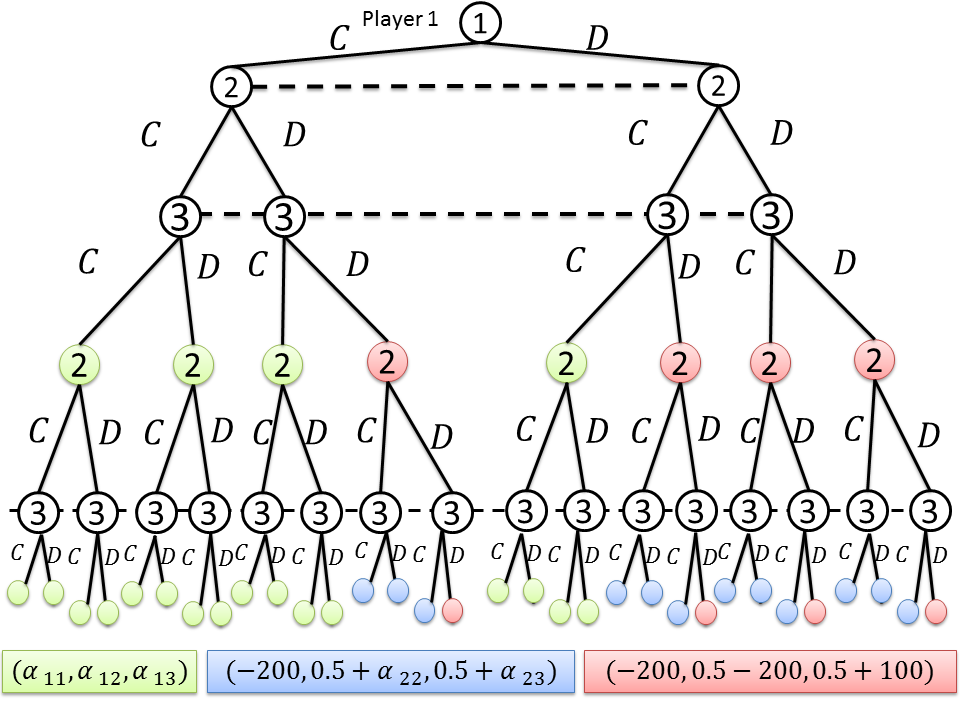
\includegraphics[scale=0.20]{Pirates1/Slide1.PNG}}
    & \num\putindeepbox[7pt]{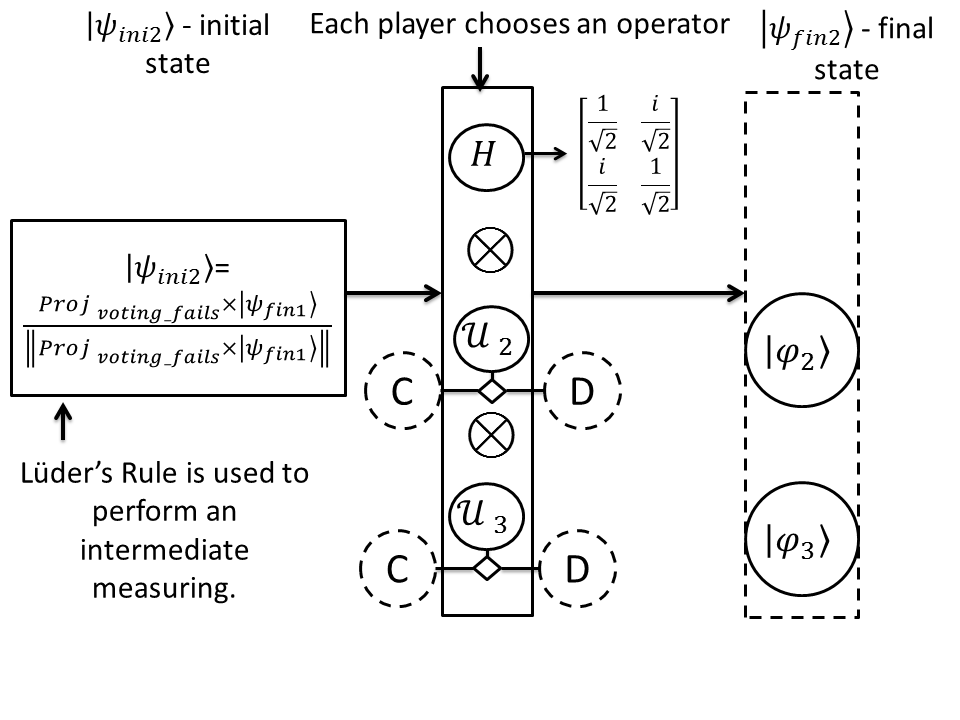
\includegraphics[scale=0.20]{Pirates1/Slide2.PNG}} \\
  \num\putindeepbox[7pt]{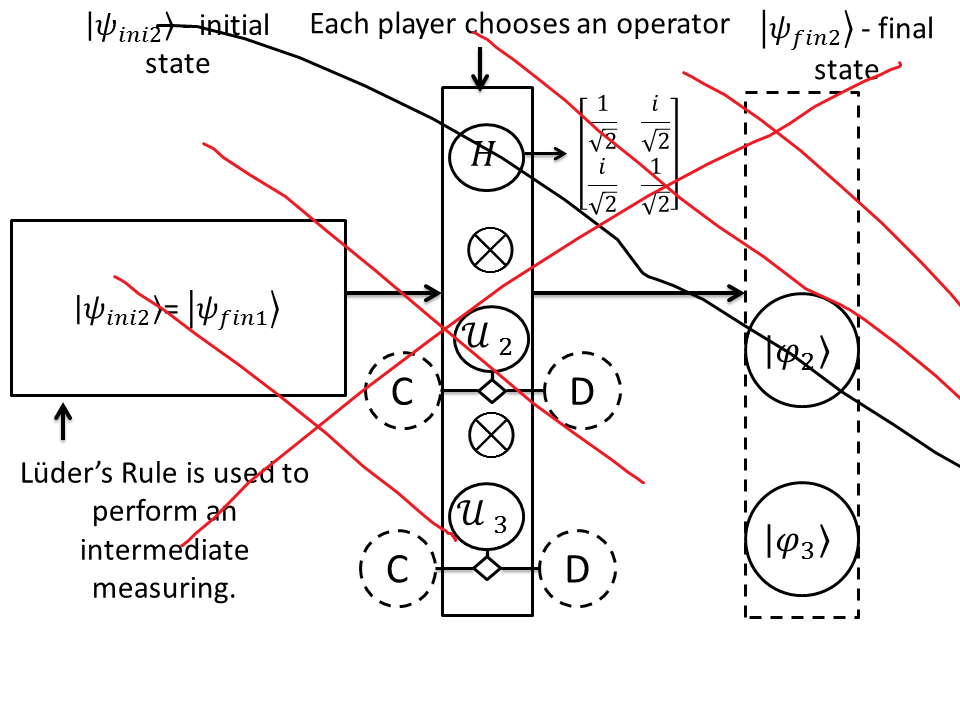
\includegraphics[scale=0.20]{Pirates1/Slide3.PNG}}
    & \num\putindeepbox[7pt]{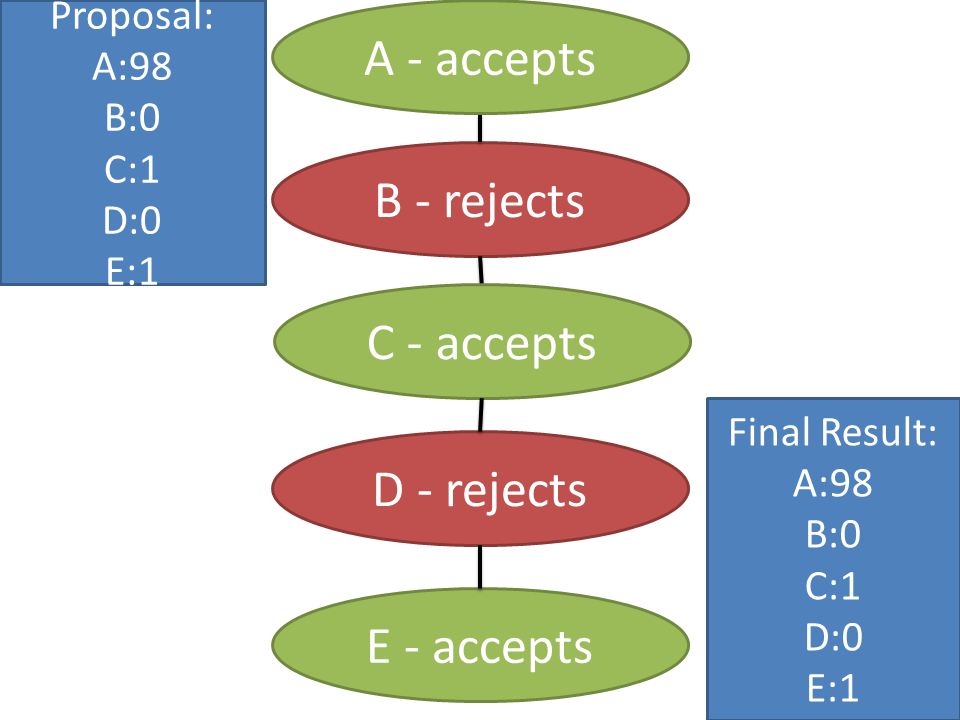
\includegraphics[scale=0.20]{Pirates1/Slide4.PNG}} \\
\end{tabular}
\caption{The equilibrium for the Pitrate Game can be found through backward induction. From a), where there's only two pirates left, to d), that corresponds to the initial problem we define the best response.}
\label{tab:piratas_m}
\end{center}
 \end{table}

When applying this reasoning to the three pirate move, as pirate C knows she needs one more vote to pass her proposal and avoiding death, she will offer the minimum amount of coins that will make pirate E better off than if it comes to the last stage with two pirates. This means that pirate C will offer 1 gold coin to pirate E, and keep the remaining 99 coins. 

With 4 pirates, B would rather bribe pirate D with 1 gold coin, because E would rather like climb on the hierarchy and getting the same payoff. Finaly, with 5 pirates the captain (A), will keep 98 gold coins and rely on pirate C and E to vote in favor of the proposal, by giving 1 gold coin each.

We can generalize this problem for $N$ pirate. If we assign a number to each pirate, where the captain is number 1 and the lower the number the higher the rank. If the number of coins is superior to the number of pirates, the equilibrium will have the captain (highest ranking pirate), giving a gold coin to each odd pirate, in case the number of players alive is odd, while keeping the rest to herself. When we have a even number of players the captain will assign a gold peice to each pirate with a even number, and the the remaining coins to herself.

\subsection{Hipothesys}
\label{subsec:qhipothesis}

The original Pirate Game is posed from the point of view of the captain. How should she allocate the treasure to the crew in order to maximize her payoff.
We can find the a equilibrium to the original Pirates Game and, while the solution may seem unexpected at first sight, it is fully described using backwards induction. 

When modeling this problem from a quantum theory perspective we are faced with some questions. The main difference from the original problem will rely on how the system is set up. Will the initial conditions provide different equilibria sittuations? Is there a condition where we are left with the classical problem? Is it possible for a captain, in a situation where we have more than two pirates left, to aquire all the coins?





\subsection{Quantum considerations}
\label{subsec:description_2}

In order to model the problem we will start by defining it using the definition of quantum game ($\Gamma$), referred in \ref{eq:quantum_game_six_tuple}, Section \ref{sec:background_quantum_game_theory}. 

We want to keep the problem as close to the original as possible. Thus we will analyse the game from the point of view of the captain. Will her best response change?

In terms of mechanics and steps, this problem could be described using $3$ players and later extended to any number $N$ of players. 

We begin by assigning an offset to each pirate (in order to identify her), as in the Section \label{subsec:description}. The captain is number $1$ and the lower the number the higher the rank. 

Each player will be able to manipulate a qubit in the system, in this case $\vert\varphi_{1}\rangle,\:\vert\varphi_{2}\rangle,$ and $\vert\varphi_{3}\rangle$, with one of two operators \ref{eq:operators_piratas_quanticos}. The two operators will correspond to the action of voting ``Yes'' or to Cooperate, and voting ``No'', meaning that they will not accept the proposal. For the defection operator ($D$), we chose one of Pauli's Operators - the Bit-flip operator. The cooperation operator will be represented by the Identity operator. 

\begin{equation}
\label{eq:operators_piratas_quanticos}
\mathcal{U}_{i} = \begin{cases}
C = o_{i0}=\left[\begin{array}{cc}
1 & 0\\
0 & 1
\end{array}\right]\\
D = o_{i1}=\left[\begin{array}{cc}
0 & 1\\
1 & 0
\end{array}\right]
\end{cases} , i \in \{ 1, 2, 3 \}
\end{equation}

The initial system will be set up by defining an entanglement coefficient $\gamma$, that affect the way the three qubits are related \ref{eq:estado_inicial_pg}.
 
\begin{equation}
\label{eq:estado_inicial_pg}
\vert \psi_{in}(\gamma) \rangle= cos( \gamma)\vert 000\rangle+ isen(\gamma)\vert 111 \rangle, \gamma \in (0,\pi)
\end{equation}

The highest ranking pirate in the hierarchy will be responsible to make a proposal to divide the 100 gold coins. This proposal is modelled as choosing some parameters for the payoff functionals for every player, according to some rules. These parameters will be $\alpha_{1}, \alpha_{2}, \alpha_{3}$, and they will obey to the Equation \ref{eq:goodss}.

\begin{equation}
\label{eq:goodss}
\sum_{i=1}^{3}\alpha_{i}=100\wedge\alpha_{i}\in\mathbb{N}_{0}
\end{equation}

The proposed goods allocation will be executed if there is a majority (or a tie), in the voting step. A step in the game consists on the highest ranking pirate defining a proposal and the subsequent vote, where all players choose simultaneously an operator. If the proposal is rejected the captain will be thrown off board, to account for the fact that this situation is very undesirable for the captain he will receive a negative payoff of $-200$.

\begin{quotation}
``When the result is indifferent the pirates prefer to throw another pirate overboard and thus climbing in the hierarchy.''
\end{quotation}

We will account for this preference by assigning an expected value of half a coin ($0.5$), to the payoff of the players that will climb on the hierarchy if the voting fails.

Each step will be identified by the offset of the highest ranking pirate. So with $3$ pirates we start with step $1$, if the voting is rejected we will get to step $2$, where 1 vote is enough to pass a proposal.

After the voting, we will use the L\"{u}der's Rule to prepare the system for the next step. In the original problem the problem with $2$ players is a subproblem of a problem with $3$ players where the first captain is killed. Our hipothesys states that the way we set up our system may provide different results, so we will try to analyse the subgame with $2$ players giving the fact that in a system with $3$ players the proposition failed. 

To analyse the step $2$,  the system will be kept in the initial dimension ($\mathcal{H}^{3}$), because of the following reasons: if we have entangled states, they won't be are separable; There may be various mappings in a lower dimension that fit the higher dimension composition. This means that the previous highest ranking player will no longer have access to the voting operators, instead she will use invariabily a symetric coin operator.


\begin{comment}

''''''Depending on the measurement outcome that occurs with probability x, the players will act on the second round. The Luders rule is applied here. The highest ranking player will no longer have access to the voting operators, instead he will only be able to manipulate de system using a symetric coin operator.

Keeping the system in a higher dimension is considered because of the following reasons: if we have entangled states, they won't be are separable, and there are various mappings to a lower dimension that fit the system composition. 


\begin{emph}
One important aspect is that the payoff functional changes

Initial state: variable to study.
Payoff functions: variable to study.
\end{emph}

\end{comment}